\documentclass{beamer}
\usepackage{ctex, amsmath, cite}
\usepackage{graphicx}


\usetheme{AnnArbor}
\usecolortheme{seagull}

\title{Geant模拟液闪探测器及本底分析}
\author{张爱强}
\date{\today}

\begin{document}
\begin{frame}
    \titlepage
\end{frame}
\begin{frame}
    \tableofcontents
\end{frame}
\section{探测器参数}
\begin{frame}
    \frametitle{探测器设计}
    \begin{block}{设计要求}
        \begin{enumerate}
            \item 10000吨的液体闪烁体探测器,球形探测器,中心有效体积为5000吨
            \item LAB为探测器材料,分子式为$C_6H_5C_nH_{2n+1}$,其中$n=12$,密度$\rho=0.863g/cm^3$
        \end{enumerate}
    \end{block}
    \begin{figure}
        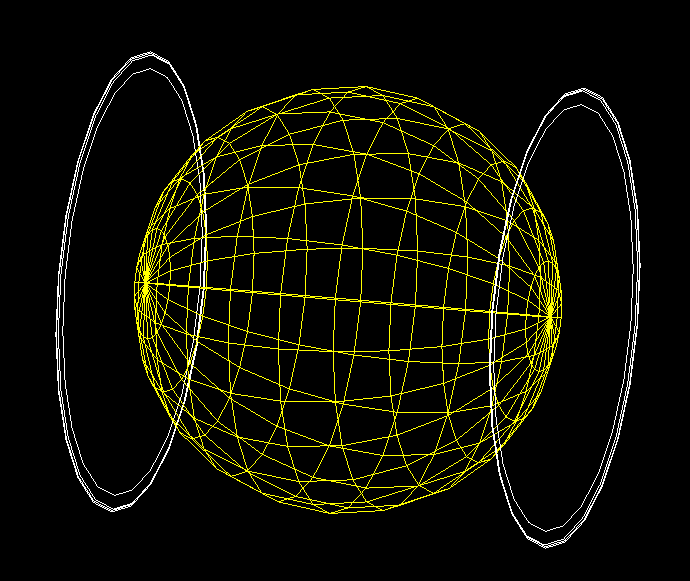
\includegraphics[width=0.5\textwidth]{figure/geometry.png}
    \end{figure}
\end{frame}
\begin{frame}
    \begin{block}{设计参数}
        探测器半径
        \[R=(\frac{3M}{4\pi\rho})^{1/3}=14.038m\]
        有效体积半径
        \[r=(\frac{3m}{4\pi\rho})^{1/3}=11.142m\]
        为了制造上的方便,精确到一位小数$R=14.1m$. 此外在液体闪烁体外层加上圆柱形的水屏蔽层$R_{water}=15m$,最外层是铅屏蔽层$R=[15.1m,15.2m]$
    \end{block}
    \begin{block}{物理过程}
        物理过程使用的是`FTFP_BERT`,已经包括了强相互作用,弱相互作用,电磁相互作用等过程。
    \end{block}
\end{frame}
\section{$\mu^-$衰变能谱模拟}
\begin{frame}
    \frametitle{$\mu^-$衰变}
    \begin{columns}
        \begin{column}{0.5\textwidth}
            \[\mu^-\to \hat{\nu}_e+\nu_{\mu}+e^-\]
            因为$\nu$反应截面较小,所以在代码中直接选择对应的粒子提取相应的能量。图为$\nu_e$能谱\cite{Armbruster:1998qi}。
            \begin{enumerate}
                \item $\mu^-$均匀分布在中心的有效体积内,均静止.实际上模拟的范围是$r<5m$
                \item 在$steppingAction$中提取$\hat{\nu_e}$,$\nu_{\mu}$,$e^-$产生时的能量,在$EventAction$中填充进$AnalysisManager$中
            \end{enumerate}
        \end{column}
        \begin{column}{0.5\textwidth}
            \begin{figure}
                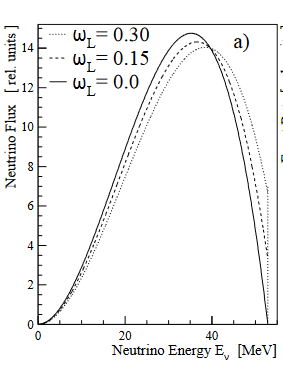
\includegraphics[width=\columnwidth]{figure/nu_eSpectra.png}
            \end{figure}
        \end{column}
    \end{columns}
\end{frame}
\begin{frame}
    \begin{figure}[h]
        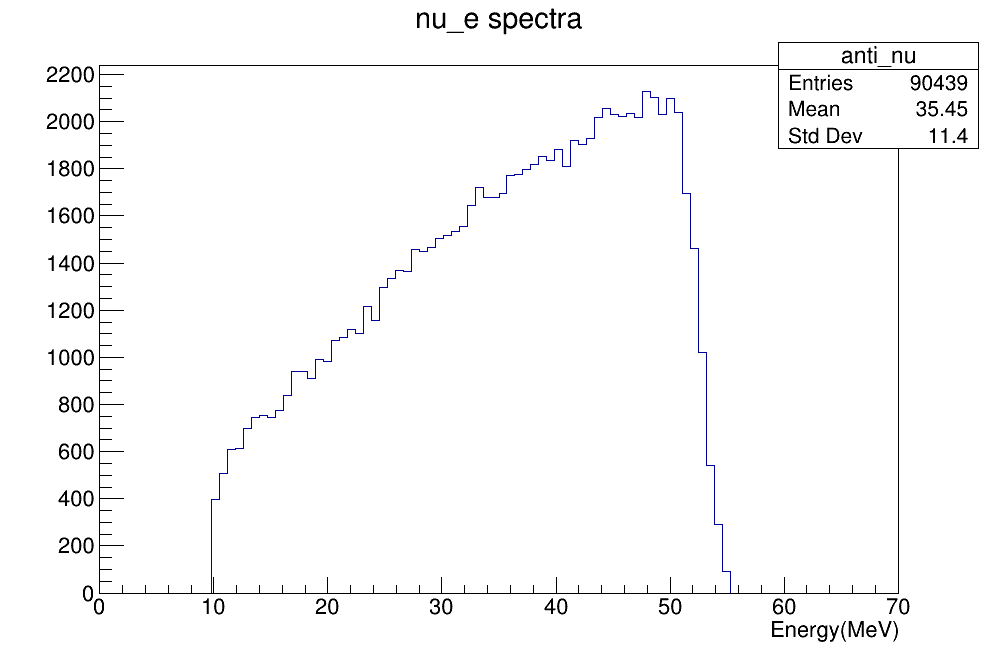
\includegraphics[width=\textwidth]{../../B2/B2b-build/signallinear.png}
    \end{figure}
    \begin{enumerate}
        \item $\nu_e$的能谱位于$0-55MeV$之间
    \end{enumerate}
\end{frame}
\begin{frame}
    \begin{figure}[h]
        \includegraphics[width=\textwidth]{../../B2/B2b-build/signallog.png}
    \end{figure}
    \begin{enumerate}
        \item 最后一张图显示末态粒子能量之和基本位于同一个位置
    \end{enumerate}
\end{frame}
\section{$n$本底能谱模拟}
\begin{frame}
    \frametitle{$n$本底}
    快中子本底来自于宇宙线$\mu$与岩石之间的作用或者一些放射性衰变产生,所以模拟过程中特意将快中子源放置在外层部位。
    在模拟中提取能量的过程中有一些问题存在。
    \begin{enumerate}
        \item $n$均匀分布在液闪探测器的外层球壳内,实际上模拟的范围是$13m<<13.5m$,动能按照指数分布$e^{\frac{E}{1GeV}}$,$0<E<10GeV$.
        \item 在$steppingAction$中提取$n$的动能,$p$的动能,$p$沉积产生时的能量,以及$p$的产生位置,在$EventAction$中填充进$AnalysisManager$中
    \end{enumerate}
\end{frame}
\begin{frame}
    \begin{figure}[h]
        \includegraphics[width=\textwidth,height=8cm]{../../B2/Bg-build/backgroundlinear_bak.png}
    \end{figure}
    \begin{enumerate}
        \item 问题1:仅提取中子动能,但是均值不正确,理论上接近$1GeV$;质子初始动能类似。
    \end{enumerate}
\end{frame}
\begin{frame}
    \begin{figure}[h]
        \includegraphics[width=\textwidth,height=8cm]{../../B2/Bg-build/backgroundlog.png}
    \end{figure}
    \begin{enumerate}
        \item 问题2:仅选择质子时发现粒子数目偏少,在剔除了动能为0的质子后。
    \end{enumerate}
\end{frame}
\section{信号本底区分}
\begin{frame}
    \frametitle{信号特征}
    \begin{enumerate}
        \item 反beta衰变的产物是$n$和$e^+$,两个产物在时间上会有一个差异,可以用符合来鉴别。
        \item 部分高能的$e^+$可能产生切伦科夫光。
        \item 产生位置选择在中心,在之前的模拟结果中分析可以得到有效体积中产生的质子数目占总数目的$0.54$,有理由肯定在考虑外界屏蔽情况下有效体积中的本底数目会更少
        \item 能量上选择低能事例$10MeV<E<60MeV$,过低能量中子本底或者其它低能噪声有影响,高于信号能谱最高能量的地方可以全部舍去。剩余部分占$0.35*054*=0.189$
    \end{enumerate}
    \begin{figure}[h]
        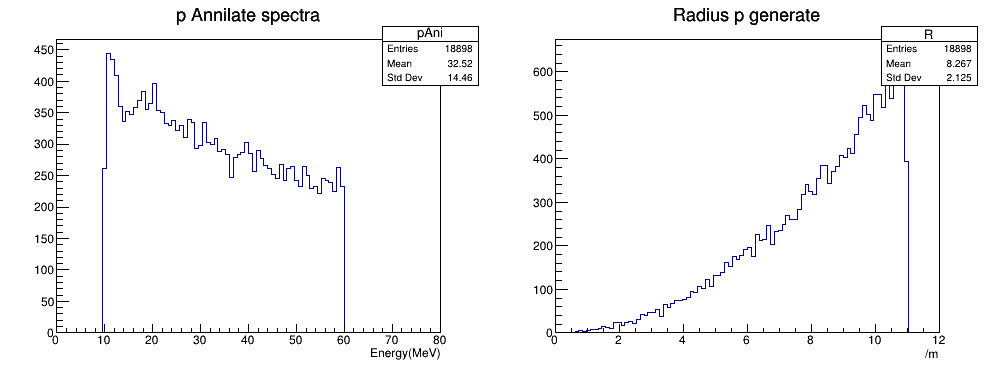
\includegraphics[width=0.8\textwidth]{../../B2/final/backgroundlinear_2.png}
    \end{figure}
\end{frame}
\begin{frame}
    \frametitle{统计方法区分粒子}
    \begin{block}{思考}
        假设事例均为本底,那么$E$一定服从指数分布。每个探测到的事例对应一个概率$p(E)$,相乘可以获得极大似然函数。可以用指数分布拟合,检验拟合优度。

        将$E$分布的区间划分成一系列的bin,每个bin有一个期待值,观测值构成的函数$\chi^2=\sum_{i=1}^{N}{\frac{(n_i-\nu_i)^2}{\nu_i}}$服从一个卡方分布
    \end{block}
\end{frame}
\section{上限确定}
\begin{frame}
    \frametitle{贝叶斯方法}
    为了避免上限估计得结果出现负值,引入Bayes概率,下面是9.54式
    \[\beta=\frac{e^{-(\nu_s^{up}+\nu_b)}\sum_0^{n_{obs}}{\frac{(\nu_s^{up}+\nu_b)^n}{n!}}}{e^{-(\nu_b)}\sum_0^{n_{obs}}{\frac{(\nu_b)^n}{n!}}}=\frac{1-F_{\chi^2}{(2(n_{s}+n_b),2(n_{obs}+1))}}{1-F_{\chi^2}{(2(n_b),2(n_{obs}+1))}}\]
    利用数值计算的方式可以给出:

    对于本底数目有365,观测数目为365,$\beta=0.1$上限估计为$32.76$;$\beta=0.05$上限估计为$38.73$
\end{frame}
\begin{frame}
    \frametitle{CLs方法}
    \[CLs=\frac{p_{s+b}}{1-p_b}=\frac{e^{-(\nu_s^{up}+\nu_b)}\sum_{0}^{n_{obs}-1}{\frac{(\nu_s^{up}+\nu_b)^n}{n!}}}{1-e^{-(\nu_b)}\sum_{n_{obs}}^{\infty}{\frac{(\nu_b)^n}{n!}}}=\frac{1-F_{\chi^2}{(2(n_{s}+n_b),2(n_{obs}))}}{1-F_{\chi^2}{(2(n_b),2(n_{obs}))}}\]
    利用数值计算的方式可以给出:

    对于本底数目有365,观测数目为365,$\beta=0.1$上限估计为$32.12$;$\beta=0.05$上限估计为$38.50$
    \begin{columns}
        \begin{column}{0.5\textwidth}
            利用MC方法模拟得到Q分布$Q=-2ln\frac{L(N_{obs},N_s+N_b)}{L(N_{obs},N_b)}$

            对于本底数目有365,观测数目为365
            
            $\beta=0.1$上限估计为$38.05$;
        \end{column}
        \begin{column}{0.5\textwidth}
            \begin{figure}[h]
                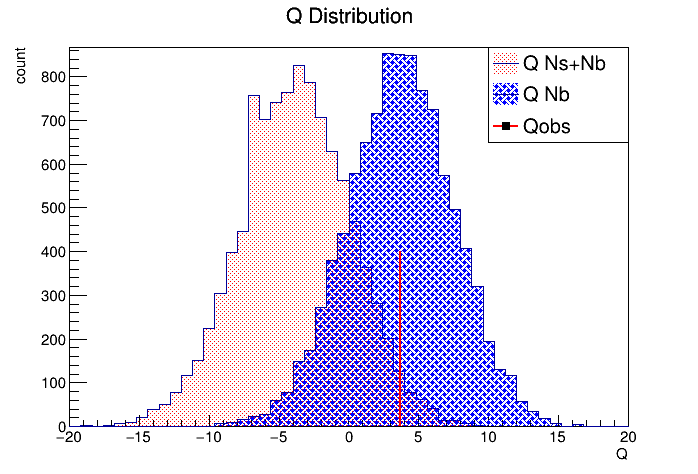
\includegraphics[width=\columnwidth]{../../B2/final/Qdist_38.png}
            \end{figure}
        \end{column}
    \end{columns}
\end{frame}

\section{参考文献及致谢}
\begin{frame}[allowframebreaks]{References}
	\bibliographystyle{plain}
	%\bibliographystyle{IEEE}
	%\bibliography{mybeamer} also works
    \bibliography{./final}
    


    感谢\texttt{康有恩},\texttt{张炳韬},\texttt{杨宇祺}和我讨论相关问题以及代码上的指点,收获很多。
\end{frame}
\begin{frame}
    \frametitle{Feldman Couison方法}
    \begin{columns}
        \begin{column}{0.5\textwidth}
            观测量概率密度函数$P(x|\mu)$,$\mu$是估计量,$x$是观测值。

            对于某个x,可以找到$\mu_{best}$使得$P$最大。那么对于$x$,定义似然比$R(x,\mu)=\frac{P(x|\mu)}{P(x|\mu_{best})}$

            对于确定的$\mu$值,可以计算对应的x的置信区间:计算不同x值对应的$P(x|\mu)$,按照上一步的R值排序,计算前面最大部分的R对应P值的和使得
            \[\sum_r{P(x|\mu)}>\gamma\]
            然后选择出被选择出的x中最大值与最小值对应于x的置信区间。

            结合实际观测的值x给出估计得$\mu$的上下限。
        \end{column}
        \begin{column}{0.5\textwidth}
            \begin{figure}[h]
                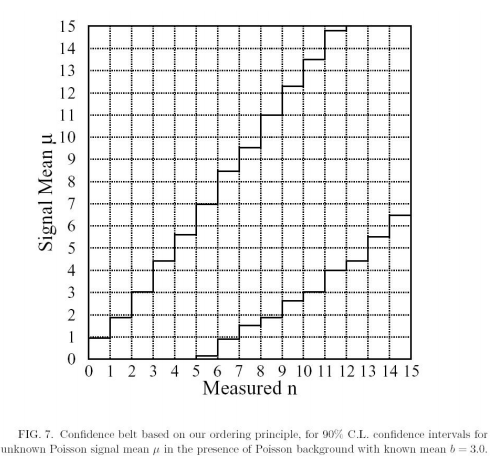
\includegraphics[width=\columnwidth]{figure/fc.png}
            \end{figure}
        \end{column}
    \end{columns}
\end{frame}
\end{document}